\documentclass{article}
% set up the page formatting
\usepackage[a4paper, portrait, margin=2.5cm]{geometry}
\usepackage{multicol}
\usepackage{fancyhdr}
\usepackage{graphicx}
\usepackage{float}

% allow for table of contents to have clickable links
\usepackage{hyperref}

% editable bits
\title{\vspace{-1.5cm}CS261 Group 29 Report}
\author{Ani Bitri, Krister Hughes, Thomas Phuong, Eshan Sharif, Josh Turner, Antoni Zyla}
\date{January 2025}
\fancyfoot[L]{Report}
\fancyfoot[R]{\thepage}

\begin{document}
    \maketitle

    \section{Preface}

    Dorset Software tasked our team with creating a traffic junction simulator. And we fucking did it.

    Dorset Software has tasked our team with the creation of a traffic junction simulator which will be used for the modelling of traffic junctions on various parameters. The system provides data on how these configurations
    affect the traffic flow and the overall efficiency of the junction in comparison to other configurations.

    This document explains the development process of the system and provide an explanation to the key changes and decisions made throughout the implementation of the prototype. Furthermore,
    it will give an insight into the algorithms and formulas used to calculate the traffic flow and efficiency of the junctions.


    \section{System Overview}

    \subsection{Purpose}

    Our system is a traffic junction simulator intended to be used by traffic engineers, urban planners and district governments to model and analyse the efficiency of different traffic junction configurations. The
    system includes a frontend interface for users to input their desired configurations, a simulation page to visualise the traffic flow and a results page to display the metrics of the simulation.

    \subsection{Developer Tools Used}

    The sytem was developed using Python and a few of its libraries. This allowed for easier transition between the frontend and backend of the system. The
    fronted was developed using PyQT5 for the GUI and MatPlotLib for aid in the Visualisation of the results.

    Our team also utilised GitHub for version control and better collaboration between team members.

    \subsection{User Interaction}

    The system is designed to be user-friendly and intuitive. When the application first opens, the user is greeted with the Home page where it displays the overview of the application and have the option to either exit to application or go to the "Input Parameters" page.
    page where they can input the desired parameters for the simulation.

    \subsection{System Architecture and Interaction}


    \section{Modifications}


    \section{Algorithms and Formulas}

    \subsection{Semaphores}

    \subsection{Traffic Flow}

    \subsection{Calculating Metrics}

    \subsection{Overall Score}


    \section{Frontend}

    \subsection{User Interface Design}
    The previous interface design combined the inputs, simulation, and results onto a single screen where you could tab between inputs and parameters. While this worked,
    a few issues arose when implementing it, such as, cluttered visuals, reduced usability, and a limited possibility of expansion. To address these newly found issues,
    instead of tabbing between the inputs and parameters pages, we made it so the inputs and parameters, the simulation, and results were given their own unique tab to
    function on. As a results of implementing the project this way, we found key advantages present in this layout compared to the previous one.

    \subsubsection{Improved Organisation}
    By separating the inputs, simulation, and results into distinct tabs, users can focus on one aspect of the interface at a time. This tabbed approach also enhances
    the workflow efficiency of the user and gives the user a natural progression to follow between data entry to simulation execution and results analysis.

    \subsubsection{Reduced Clutter}
    The previous design displayed all elements of our user interface on one screen, making it visually overwhelming and difficult to navigate. The new design split of
    the interface, allowing the user to interact with each section independently, reducing the visual overload and improving the overall ease of use.

    \subsubsection{Increased Space for Additional Features}
    The old layout restricted the ability of add new functionalities due to space constraints as all three segments were on one page. By utilising the tab-based system,
    we have created for room for additional features such as adding graphs to the results page.

    \subsection{Home Page}

    The user is first greeted with the home page where some general information about the system is displayed. The user can then click the "Go to Input Parameters" button to go to the Inputs Page
    or click the "Exit" button to exit the application. The image below shows the home page of the system:

    \begin{figure}[H]
        \centering
        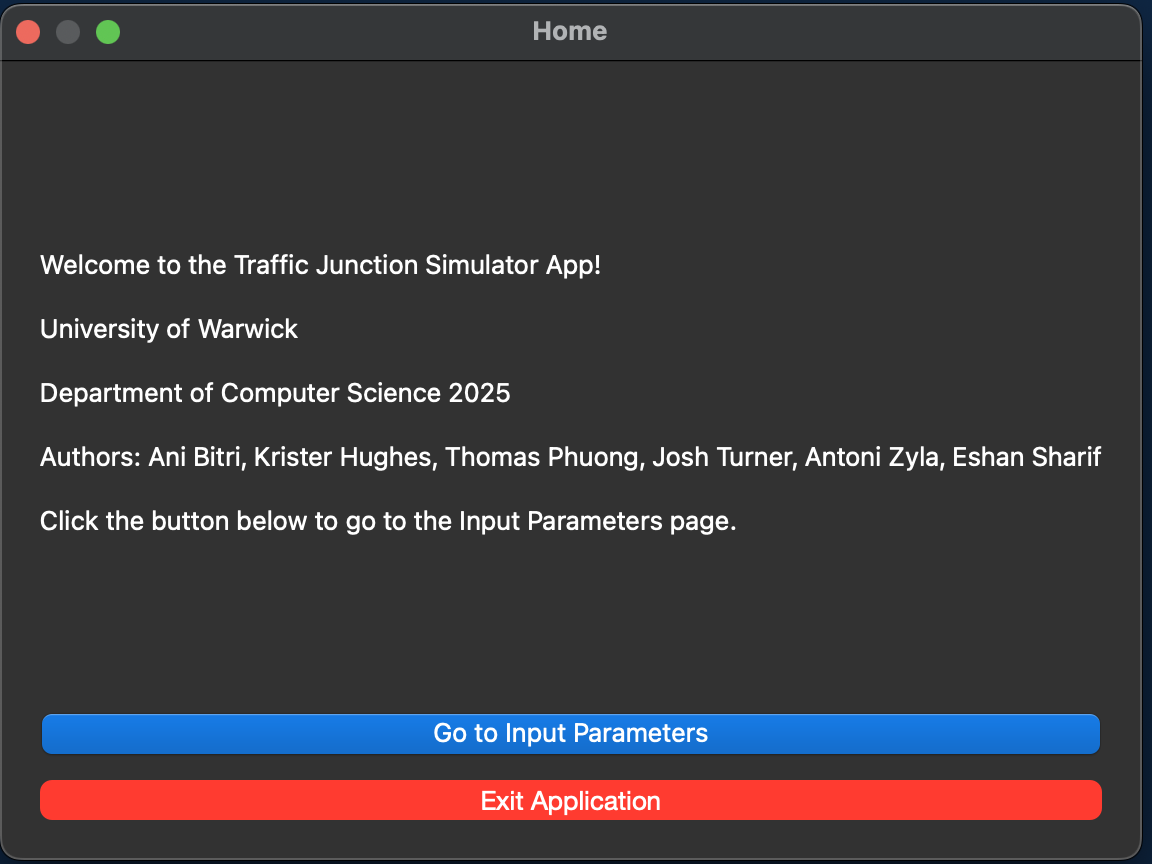
\includegraphics[width=7cm]{homepage.png}
        \caption{Home Page of the System}
        \label{fig:homepage}
    \end{figure}

    \subsection{Input and Validation Page}

    The Input Page provides a structured interface for configuring traffic flow conditions. The layout of the Input Parameters page made use of a grid and box layout to organise the input boxes for each junction. The widget uses PyQt's QScrollArea to allow the user to scroll through the multiple junction configurations, where each one of them
    is contained in a QGroupBox and stored as JunctionInputAndParameterWidget. Each JunctionInputAndParameterWidget contains 4 QGroupBoxes, one for each direction of traffic flow stored as RoadGroupWidget. Each RoadGroupWidget contains the input fields for the
    traffic flow, number of lanes, dedicated lanes, such as bus lanes and bus lane configuration, left turn lane and right turn lane; and also a priority input field. The image below shows the input page of the system:

    \begin{figure}[h!]
        \centering
        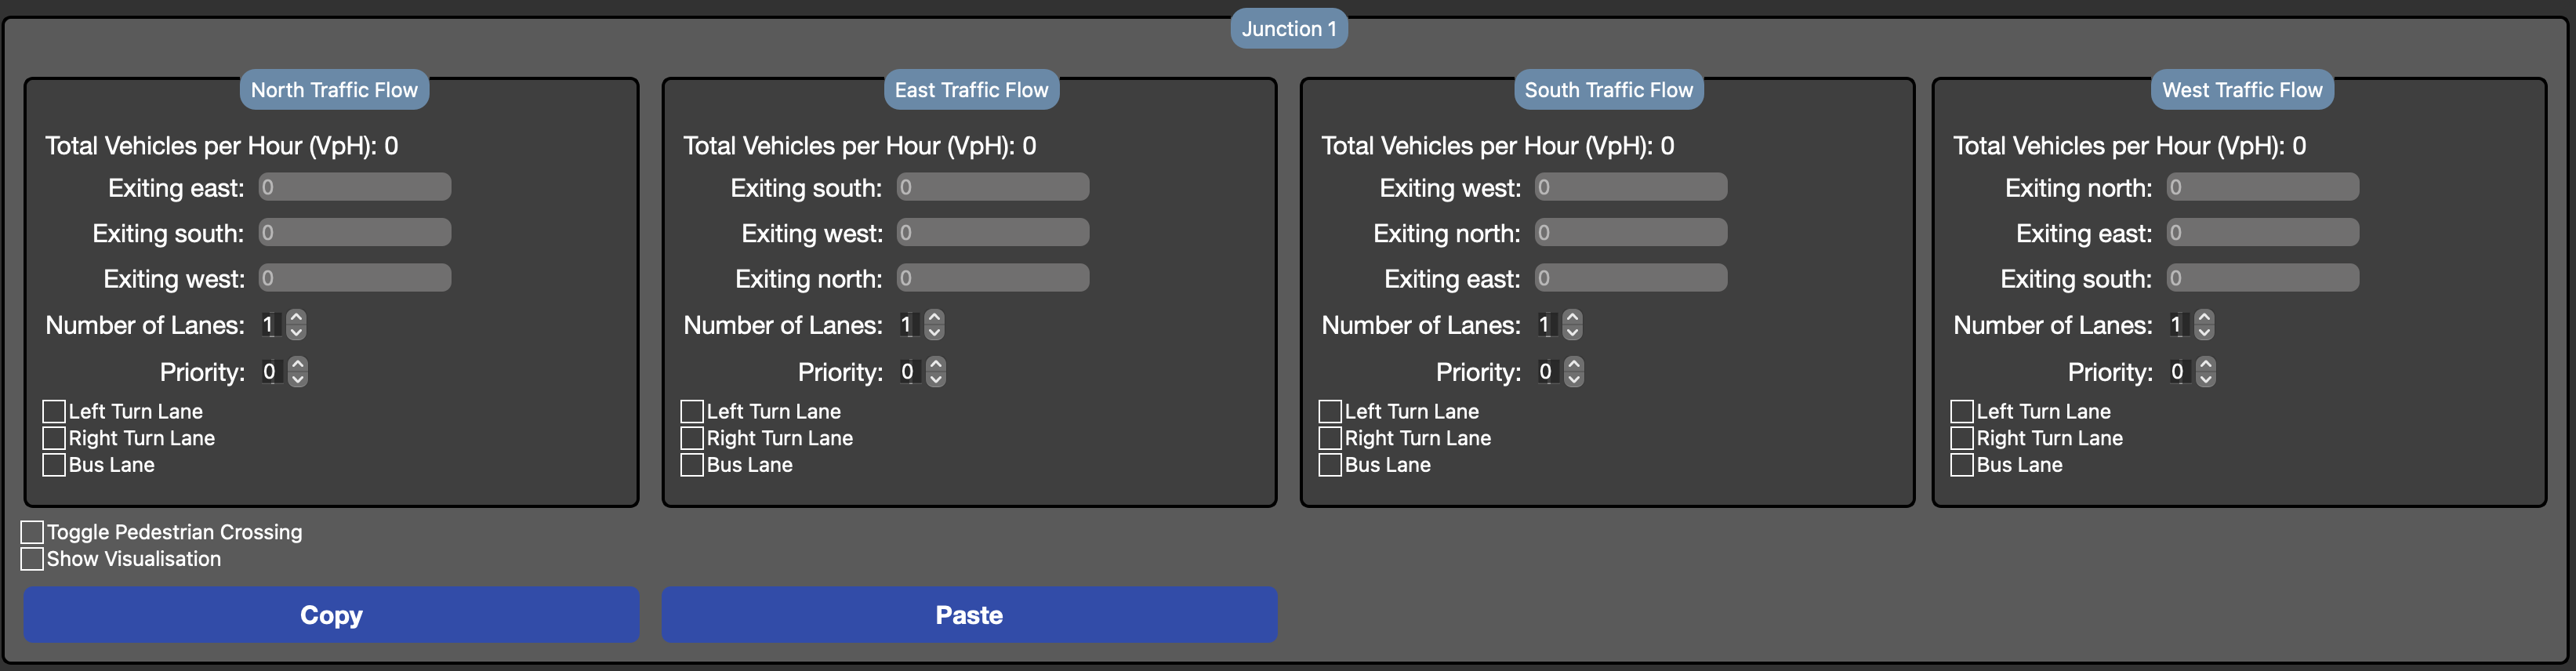
\includegraphics[width=\textwidth]{parameter.png}
        \caption{Illustration of the Input Box}
        \label{fig:parameter}
    \end{figure}

    The JunctionInputAndParameterWidget also contains two checkboxes for the user to select whether they want to add pedestrian crossing options and whether they want to see the updates on the junction on real time. A visual representation of the
    junction is displayed on the right side of the parent box, which updates in real time as the user inputs the parameters. Furthermore, the parent box contains copy and paste buttons, where the user can copy the data entered
    in the first junction configuration, and reuse it in the other configurations. The image below shows the visual representation:

    \begin{figure}[H]
        \centering
        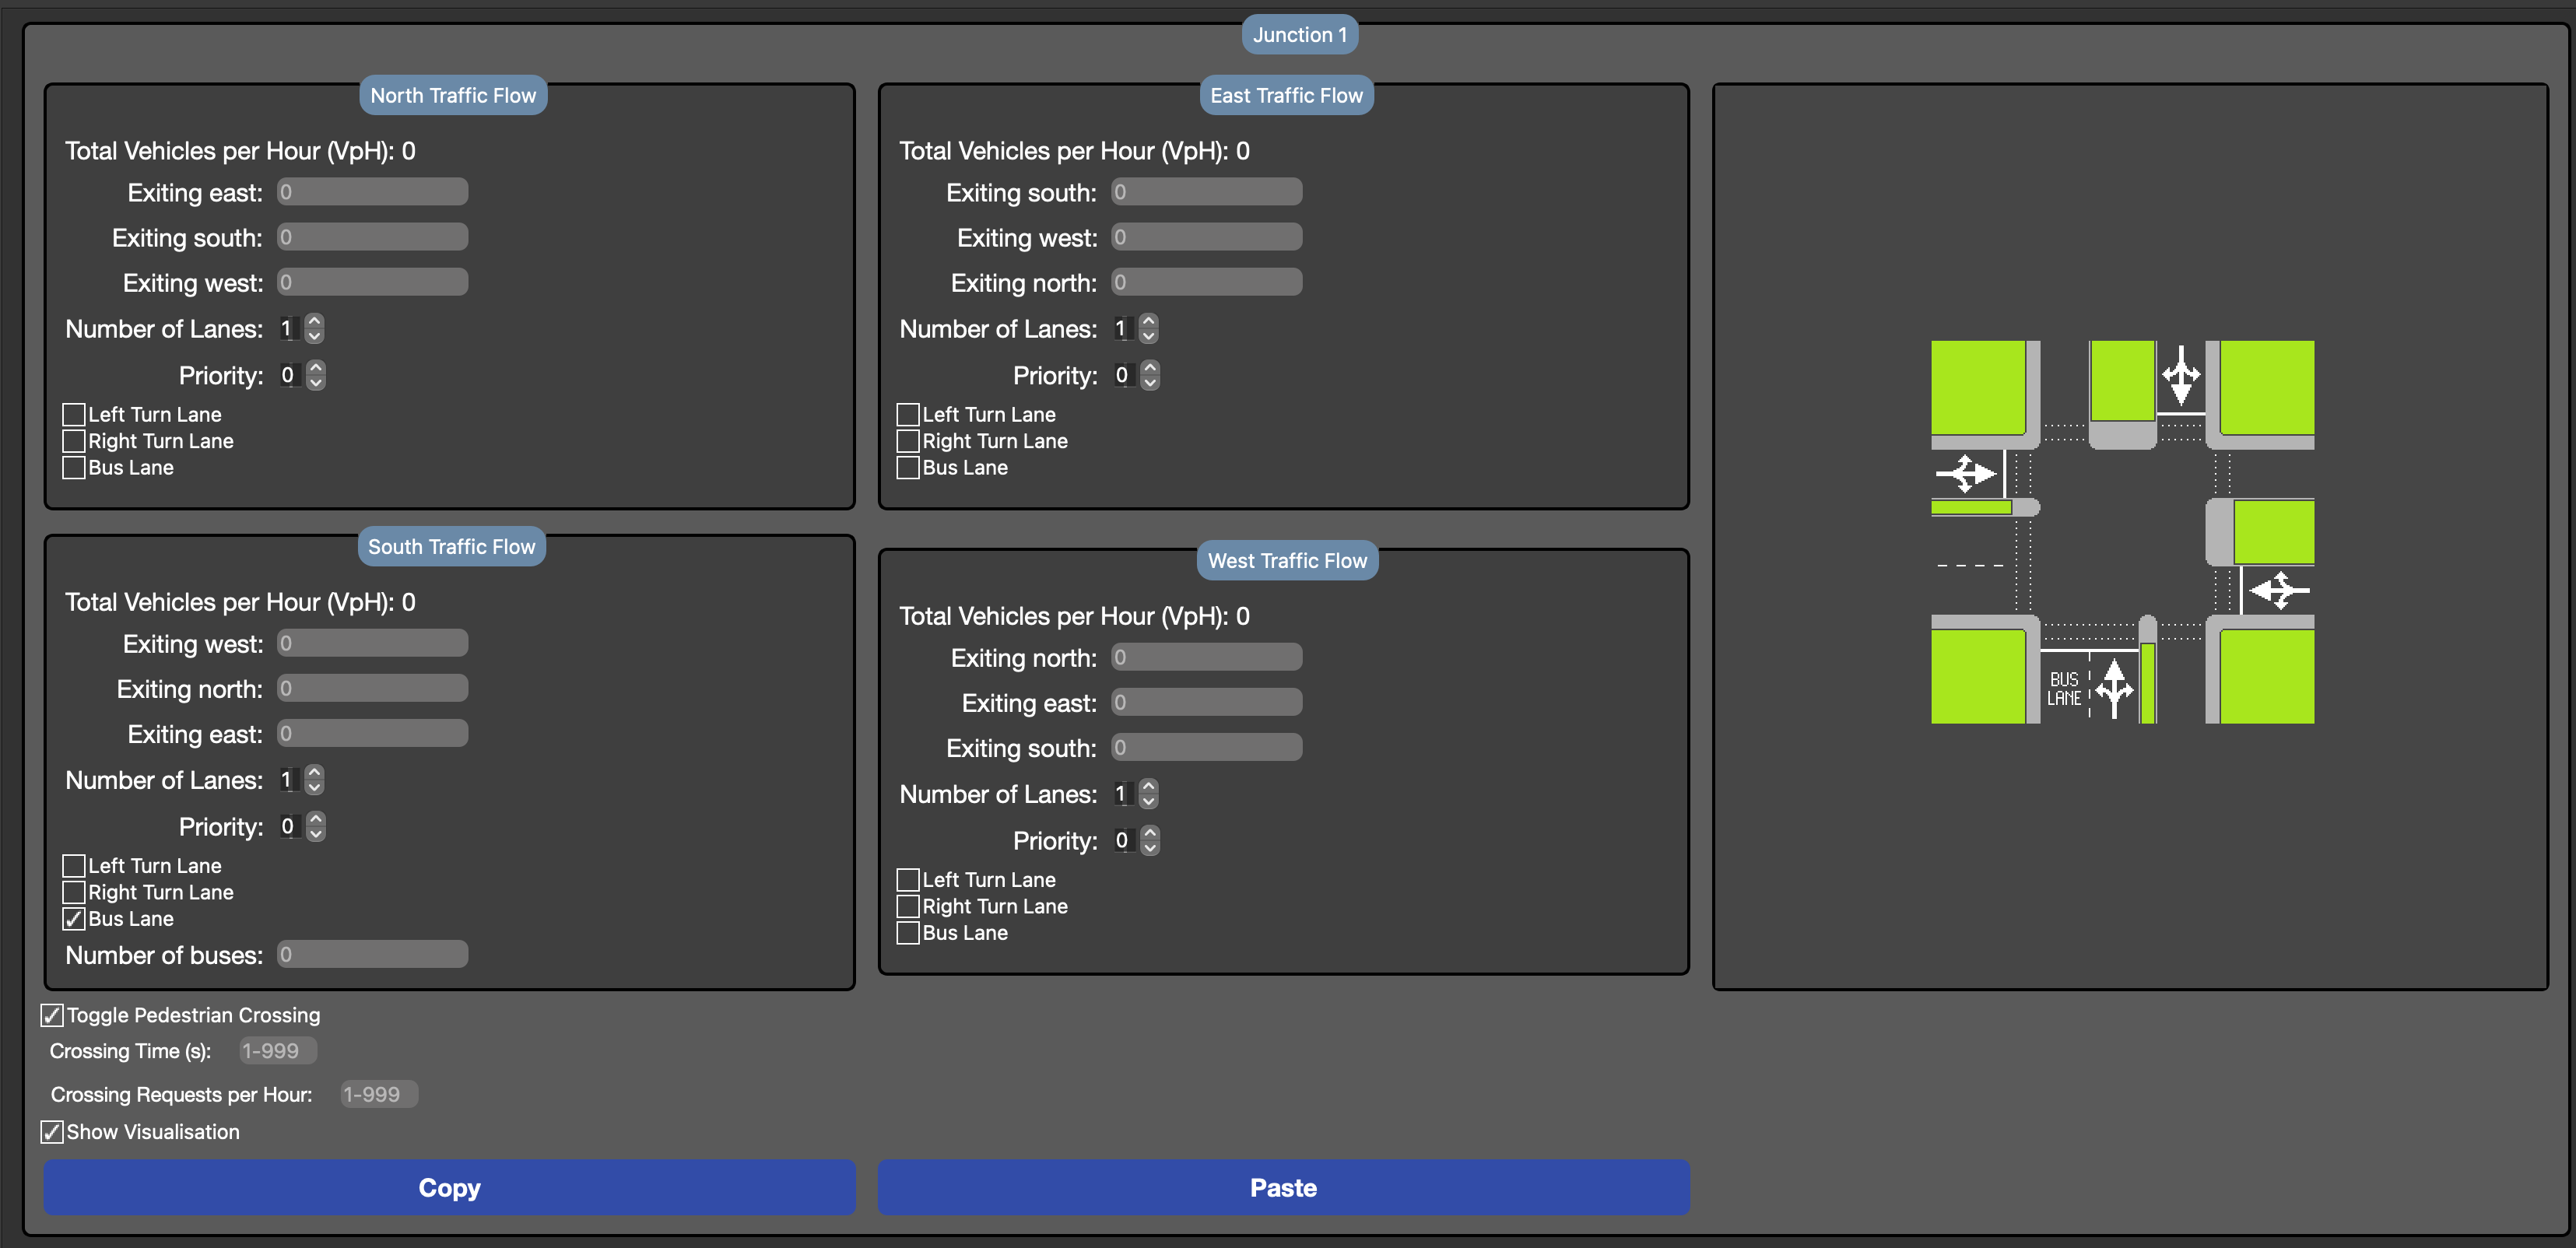
\includegraphics[width=\textwidth]{inputExtra.png}
        \caption{Illustration of the Input Box with additional options}
        \label{fig:inputExtra}
    \end{figure}

    Once the user has input the desired parameters, they can click the "Start Simulation" button at the bottom of the page to send the data to the backend and start the simulation. After the user has clicked the "Start Simulation" button, they
    will be taken to the Results Page where the results of the simulation will be displayed.

        \subsubsection{Visualisation}
            In the initial design document, the implementation of the junction visualization was left fairly open to allow for future revisions, as permitted by the modified version of the Waterfall Methodology used by the group. Once a basic input window had been created, the constraints (Such as left lanes and bus lanes being mutually exclusive) on the junction became clearer; this then aided with design of the classes involved:
            \begin{figure}[H]
                \centering
                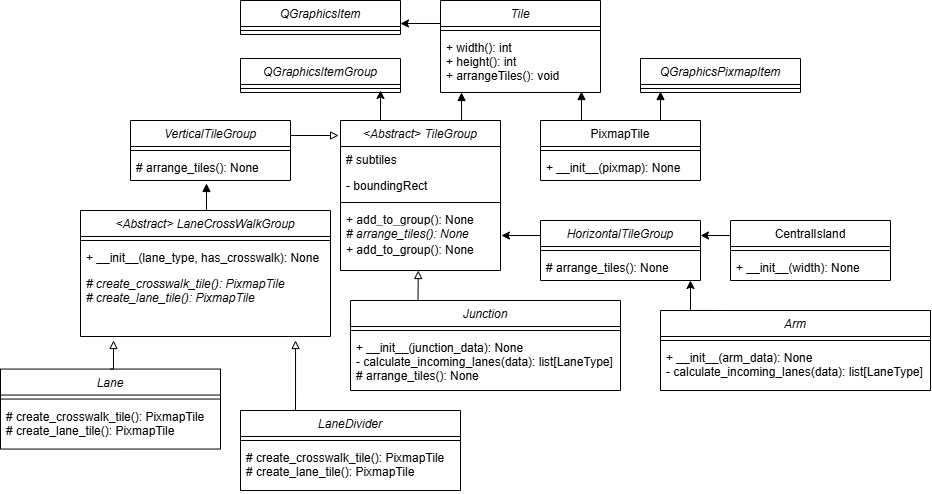
\includegraphics[width=\textwidth]{visualisation_class.png}
                \caption{Class diagram for the visualisation}
                \label{fig:visualisation_class}
            \end{figure}
            The overall structure was made to be hierarchical so that each layer could independently create and position the Tiles that they contained. Having both TileGroups and PixmapTiles inherit from Tile was intended to provide a layer of abstraction that would simplify the code.
            \begin{figure}[H]
                \centering
                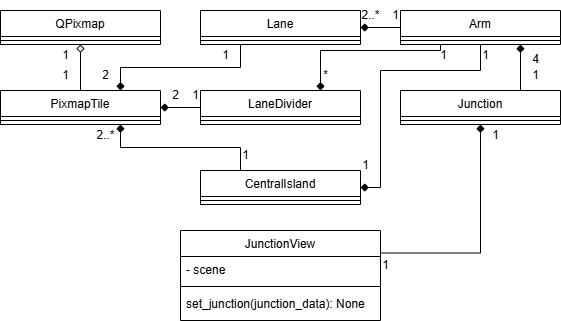
\includegraphics[width=0.6\textwidth]{visualisation_relationship.png}
                \caption{Relationships between classes in the visualisation}
                \label{fig:visualisation_relationship}
            \end{figure}
            When implementing this design for the implementation, the team realised that it was inefficient to create a QPixmap for each tile in the image. This was because for some junction configurations there would be as many as one hundred and fifty QPixmaps created each time the junction was updated. To increase the efficiency, a class named Pixmap was created which held a single copy of each QPixmap. These QPixmaps are persistent between updates so only need to be created once when they are first needed.\\

            The visualisation ended up meeting requirement 12 as it updates in real time as can be seen in the Dragon's Den video; however it was decided not to complete requirement 10 as this could have made the visualisation too cluttered, and could potentially be unintuitive to the user.
        
        \subsubsection{Copy and Paste}
            Although not in the origin design, the team decided to add copy and paste buttons as a quality of life improvement for the user.
            Before being implemented, comparing two junctions with the same flow rates required all twelve values to be copied manually from one junction to another; however, with the copy and paste button not only can these be copied with two clicks, but all other configurations for that junction are copied as well. 
            This significantly improves the efficiency with which the user can compare two junctions with minor differences (Likely a common use case for this application).



    \subsection{Results Page}

    The Results Page initially displays a divided design using QGridLayout, a 2x2 grid where each cell is a QGroupBox planned to contain result information about the traffic flow for each direction, but initially,
    they display instructions on how the user can generate the results and how they they will be displayed. The image below shows the initial state of a box in the results page:

    \begin{figure}[H]
        \centering
        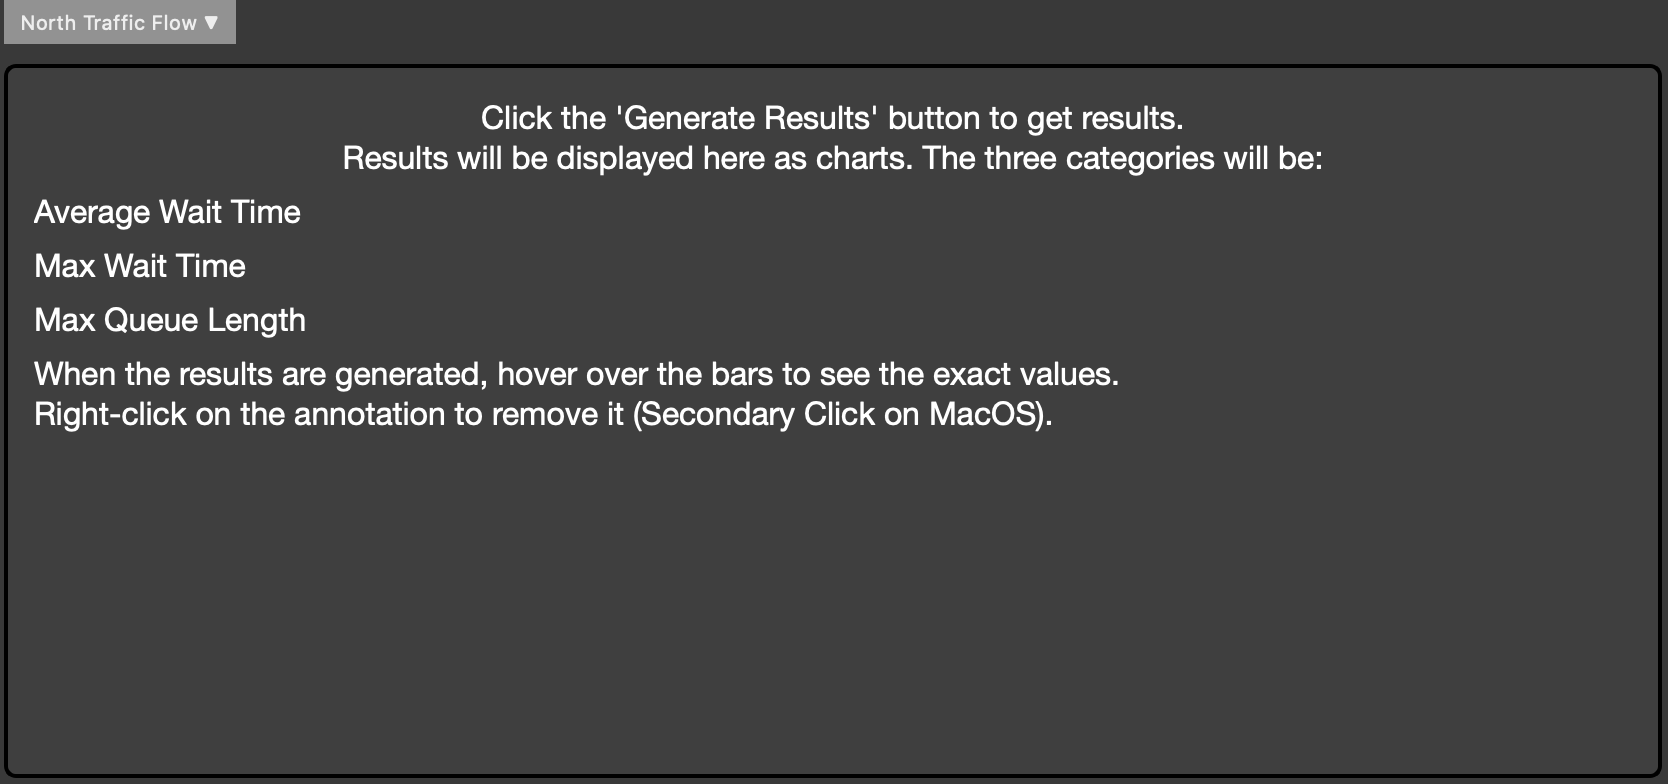
\includegraphics[width=\textwidth]{results1.png}
        \caption{Illustration of the initial state of a box in Results Page}
        \label{fig:results1}
    \end{figure}

    Once the user has generated the results, the boxes will display the metrics of the simulation on bar charts, where for the results categories (Max Queue Length, Average Wait, and Max Wait)
    each bar represents a different junction configuration. While the cursor is hovering over a bar, the user will be able to see the exact value of the metric. As instructed in the initial state
    of each direction box, the user can remove the annotation by right clicking over the ot (Secondary Click on MacOS). The image below shows the results page with the results of the simulation:

    \begin{figure}[H]
        \centering
        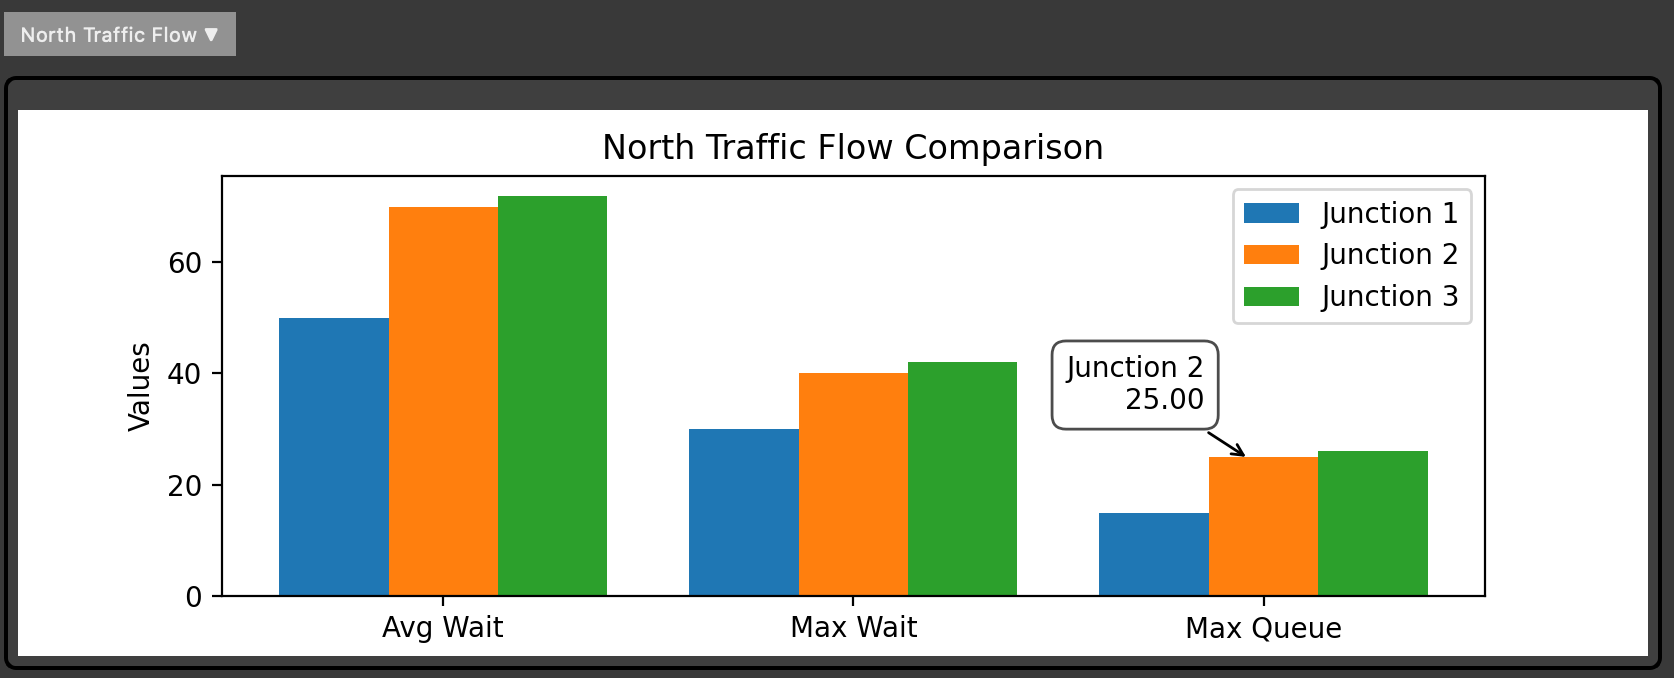
\includegraphics[width=\textwidth]{results2.png}
        \caption{Illustration of the chart with the results of the simulation for 3 different junction configurations}
        \label{fig:results2}
    \end{figure}

    The results set is retrievied as a 3D list from the backend, where te first dimension represents tje junction configuration, the second dimension represents the direction of the traffic flow, and the third dimension represents the metrics. The overall scores
    for each junction are saved in the last index of the second dimension as a float. The image below represents the structure of the results set:

    \begin{figure}[H]
        \centering
        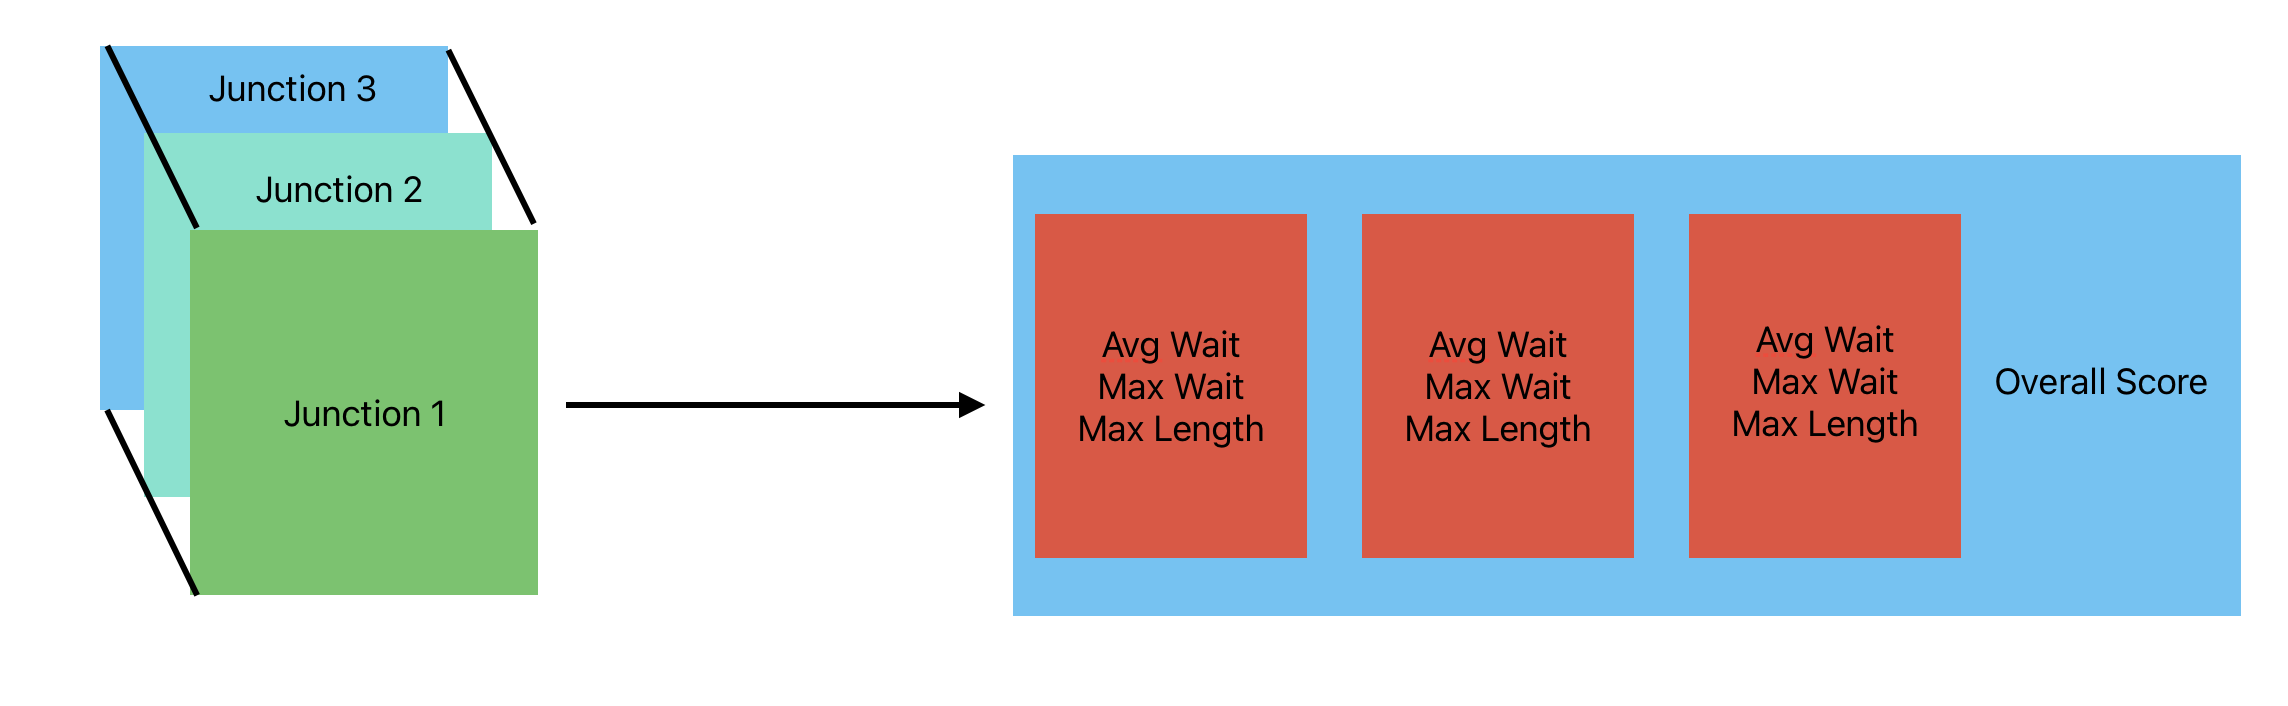
\includegraphics[width=\textwidth]{results3d.png}
        \caption{Illustration of result set structure}
        \label{fig:results3d}
    \end{figure}

    The overall scores for each junction configuration are also shown above the box layout of the directions. Depending on the number of junction configuration, the
    the overall score labels will be adjusted accordingly to the layout of the page. The image below shows the results page with the overall scores displayed:

    \begin{figure}[H]
        \centering
        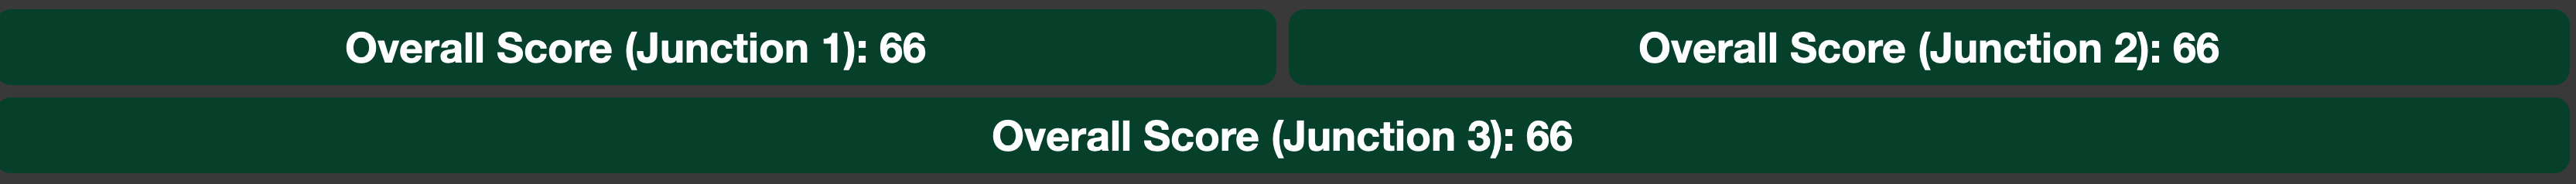
\includegraphics[width=\textwidth]{overallScores.png}
        \caption{Illustration of how the overall scores are displayed}
        \label{fig:overallScores}
    \end{figure}

    Furthermore, with the generation of the results, the user will also be able to generate a report PDF of the results. The user can do this by clicking the "Generate Report" button at the bottom of the page.
    The PDF report will contain the charts and the metrics for each direction in a text format. The next subsection will explain the PDF generation in more detail.

    \subsection{PDF generation}

    The PDF generation was implemented using the ReportLab library. It first checks whether the results have been generated (self.results\_generated). If the results exist, it prompts the user to choose a file
    location using a QFileDialog. If the user cancels the save operation, the function returns early. Otherwise, it ensures that the file has a .pdf extension before proceeding. The function then initializes a
    PDF canvas with an A4 page size and begins structuring the report by adding a title and introductory text. The function retrieves the results data from the get\_results() function and based on the number of junction
    configurations, it iterates over each direction to add a title and bar chart for each. The function then adds the overall scores and a final note before saving the PDF to the chosen file location.

    \begin{figure}[H]
        \centering
        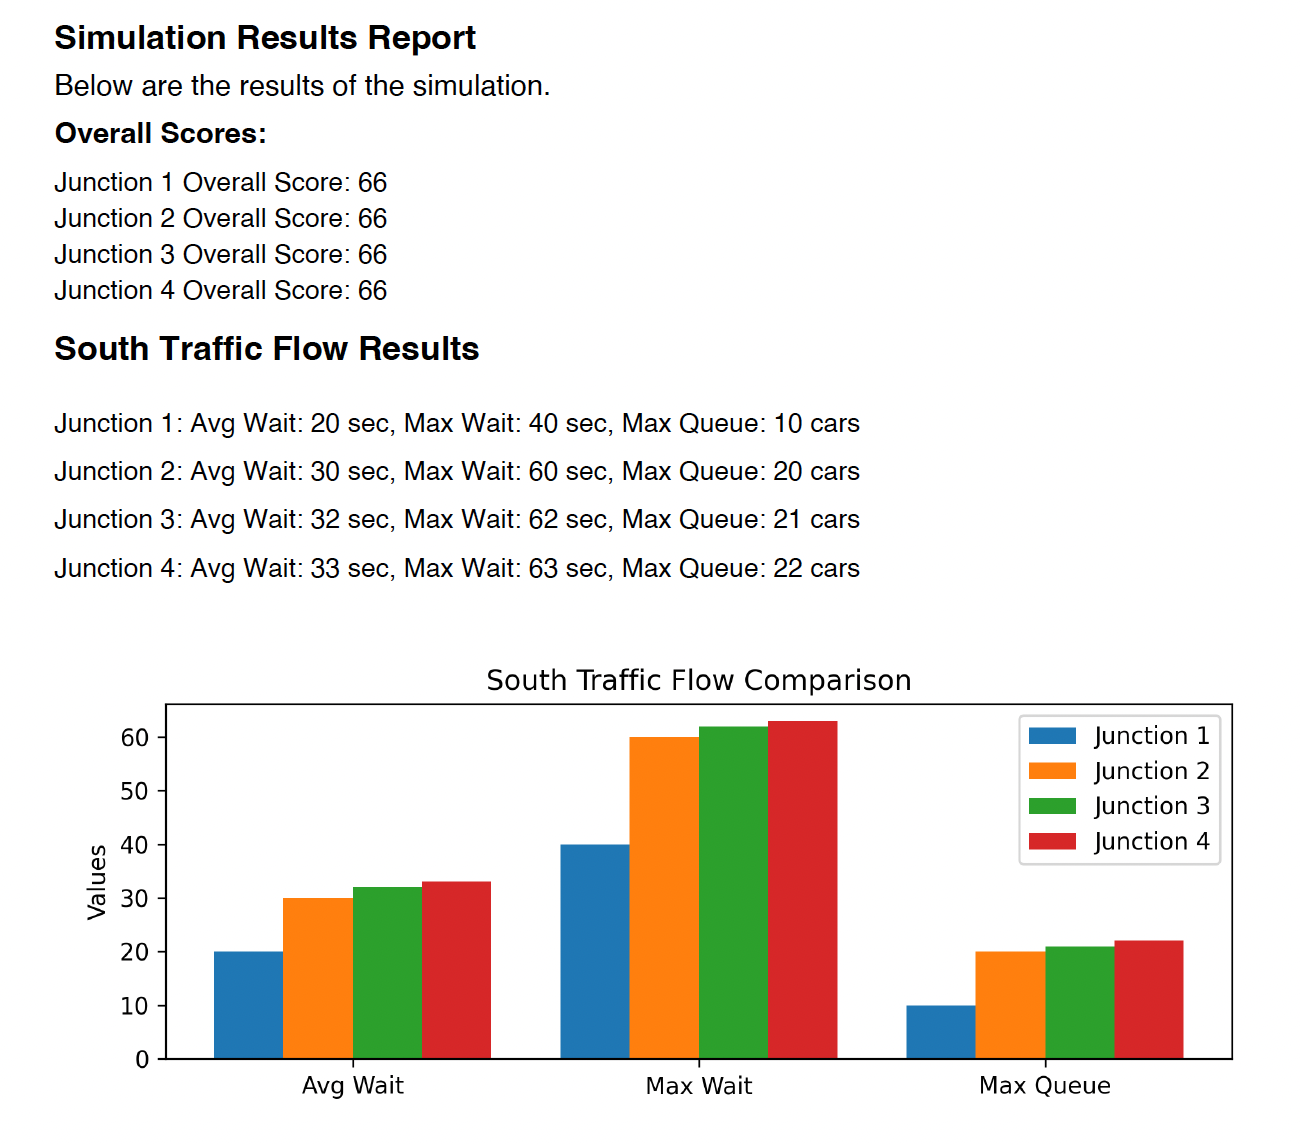
\includegraphics[width=\textwidth]{samplePDF.png}
        \caption{Sample of a PDF report generated by the system}
        \label{fig:samplePDF}
    \end{figure}

    \subsection{Error Handling}
    Within our application, there are many scenarios which require the user to input certain parameters or complete steps in a specific order. The way we handled these problems as a team were by checking and verifying the user's inputs by setting up certain constraints on the input boxes and by displaying error messages with the necessary steps to fix the issue on them.

    \subsubsection{Input Checking}
    On the Input and Parameter page we ensured that the user entered the correct inputs by having certain checks in place:
    \begin{itemize}
        \item When the user enters the VpH exiting each exit, we ensured that the input was an integer, greater or equal to 0, and had an upper bound of 999 VpH.
        \item When the user enters the number of lanes for each exit, the number had to be greater than 0, had an upper bound of 5, and was always an integer.
        \item For the Priority, we made sure that the user could only have a priority that was greater than or equal to 0, at most 4, and was an integer.
        \item If the user had chosen to add a pedestrian crossing, we made sure that the time it takes for people to cross and the number of crossing requests per hour were both greater than 0, less than 1000, and always an integer.
    \end{itemize}

    \subsubsection{Error Messages}
    There are features in our application that require the user to complete steps in a certain order.
    If the pre-requirement is not met for a certain feature, an error message will be displayed:
    \begin{itemize}
        \item If the user chooses to remove an alternate configuration without creating one in the first place, an error message will be displayed that will tell the user too add an alternate configuration before they are able to remove one.
        \item In the scenario that the user decides to generate a report PDF without generating any results, an error message would display: telling the user to press the generate results button in order to generate the results of their configuration before pressing the report button again.
        \item As the user is setting up their junction configuration, if the user does not set a suitable number of lanes, when starting the simulation an error message will display. The error message will prompt the user to change the number of lanes on the exit that has an inconsistent number of lanes and incoming traffic. The error message should tell the user which junction configuration is causing an issue and which direction of traffic flow needs to be changed.
    \end{itemize}


    \section{Backend}

    When implementing the backend we followed the class diagram and general structure as set out in the planning and
    design document, we encountered a few challenges once we got into the nitty-gritty implementation details, primarily
    regarding handling of the trafficlight timings for each lane and junction direction.

    \subsection{Data Classes}

    The system is split into the same classes as defined in the planning and design.

    \subsubsection{Params and Flowrates}

    There was a slight modification of the final implementation of both of these classes compared to the initial class
    diagram, the flowrates object no longer contains a boolean variable for driving on either side of road as this was
    not able to be implemented in the timescale of the project. The planning design specifies the flowrates object to
    encapsulate the flow rates for all directions, we decided to use different flow rates object for each cardinal
    direction as this was simpler to program. The flow rates object also includes more data about dedicated left,
    dedicated right and dedicated bus lanes, with this comes a larger constructor as well as more getters for the
    flows derived from various combinations of the above. There is also a check function included in both classes to
    check that the data is of the correct format due to the lazy type system of python

    \subsection{Simulation}

    \subsection{Results}
    The results required to be displayed by the simulator per junction were the average wait time, maximum wait time and
    maximum queue length in each direction, along with an overall score for the junction. When implementing code to
    calculate the average wait time and maximum wait time for a direction, we realised that due to only representing a
    set number of vehicles in each lane as objects and the rest of the vehicles via counters in a list called pools
    (each counter corresponding to a direction a vehicle may exit), calculating the average wait and maximum wait would
    be difficult and we could only get an approximation - vehicles couldn’t store how long they had actually been waiting,
    since they were initially represented as part of a counter. This led us to the decision to rewrite the pools from being
    a list of counters for the number of vehicles outside of the Lane objects heading in each direction, to each pool being
    a list containing Vehicle objects, all headed in the direction the pool was designated to. Along with this, the Vehicle
    class was updated to contain a time\_entered attribute, a timestamp indicating what time it arrived to the junction,
    and each Direction object had a time\_elapsed attribute (indicating the time in simulated seconds since the start of
    the simulation) to compare time\_entered to in order to work out how long a vehicle had been waiting. This was chosen
    over each vehicle having a timer keeping track of how long it had been at the junction for, since this would have
    required updating every Vehicle object every time Direction.simulateUpdate() was called, which for large flow rates
    would lead to a large amount of computation for each call, slowing the simulator down significantly.

    For the overall score, after working on it as a group, we came up with the following equation:
    $$score(J) = \sum_{d \in Dirs}\frac{flow(d) + k_P\times crossTime(d) \times crossRate(d)}{k_W (meanWait(d)+\frac{(maxWait(d))^2}{meanWait(d)}) + k_L\times maxLength(d)}$$
    The reasoning for making it dependent on the flow rate of each direction was because if a junction achieves a specific set of metrics (excluding overall score) for each direction with a certain set of flow rates, but another junction achieves that same set of metrics with a set of higher flow rates, then that second junction must be better and therefore receive a higher score. We decided to include crossing time and crossing rate in the equation since otherwise including pedestrian crossings would always lower the overall score due to preventing any traffic from flowing at given points, and in real life, pedestrian crossings do have value despite reducing how often traffic can flow. Since the score should reduce as average wait, max wait and max length increase, we decided to divide the flow rate and pedestrian crossing adjustment by average wait and max length, as well by max wait multiplied by max wait over average wait. Max wait was multiplied by this since we thought max wait should have more significance the further the value gets from average wait - for example, a junction with an average wait of 1 minute but maximum wait of an hour isn’t a very good junction. The equation also includes constants to allow for fine tuning to prefer certain junction configurations over others.


    \section{Testing}

    \subsection{Unit Testing}

    \subsection{Unit Testing}
    Unit testing was a crucial step in ensuring the accuracy and reliability of the traffic simulation system. By testing components in isolation before integrating them, we identified and resolved potential issues early. This approach validated the system’s functionality under various traffic conditions, ensured stable performance when handling large datasets, and prevented erroneous behaviours caused by unexpected inputs.

    \subsection*{Junction Class}
    The \texttt{Junction} class simulates traffic flow at intersections, managing vehicle movement and traffic light sequencing.
    \begin{itemize}
        \item The system dynamically adjusted traffic light sequencing based on real-time traffic demand. Testing confirmed that high-traffic lanes received extended green-light durations, while conflicting signals were never activated simultaneously. The logic correctly prioritised heavy-flow directions while preventing unnecessary delays for lighter-traffic lanes.
        \item Vehicle movement was simulated to verify congestion patterns, ensuring that throughput calculations reflected realistic travel times. Tests confirmed that vehicle counts decreased appropriately as cars exited the junction and that waiting times increased proportionally with higher traffic density. Data logging ensured accurate tracking of each vehicle’s journey from arrival to departure.
    \end{itemize}

    \subsection*{Lane Class}
    The \texttt{Lane} class handles vehicle queues and determines progression based on traffic signals.
    \begin{itemize}
        \item Lane capacity constraints were rigorously tested to confirm that vehicles queued in a structured manner, preventing unintended bypasses or unrealistic pile-ups. Simulations verified that vehicles moved forward only when the traffic signal allowed, with proper prioritisation for left, right, and straight movements based on sequencing rules.
        \item Empty lane optimisation was validated to ensure that the system did not perform unnecessary calculations for lanes with no vehicles. Conversely, in full-capacity scenarios, vehicles were correctly held in place until space became available, preventing system crashes or skipped queue positions.
    \end{itemize}

    \subsection*{Parameters Class}
    The \texttt{Parameters} class manages key simulation settings, including lane numbers, pedestrian crossings, and sequencing priorities.
    \begin{itemize}
        \item Input validation was tested extensively, rejecting negative lane counts, sequencing priorities outside the expected range (0-4), and unrealistic pedestrian crossing times exceeding safe thresholds. The system consistently returned appropriate error messages for incorrect inputs, ensuring that invalid configurations did not proceed to simulation.
        \item Dynamic updates to parameters were tested by modifying settings mid-simulation. The system correctly adjusted sequencing priorities, lane capacities, and pedestrian timings in real time without disrupting existing traffic states. This confirmed that parameter modifications seamlessly influenced traffic flow without requiring a system restart.
    \end{itemize}

    \subsection*{FlowRates Class}
    The \texttt{FlowRates} class defines vehicle arrival rates and enforces lane-specific traffic rules.
    \begin{itemize}
        \item The system correctly rejected negative vehicle flow rates and prevented excessively high values from distorting congestion levels. Tests confirmed that each lane’s turn restrictions were respected, ensuring that right-turn-only lanes did not process straight-traveling vehicles and vice versa.
        \item Stress testing simulated extreme cases, including intersections with zero traffic and junctions with over 1000 vehicles per hour in a single direction. The system maintained stable performance, ensuring that congestion did not overflow into unrealistic queue lengths and that vehicle processing remained within expected real-world limits.
    \end{itemize}

    \subsection*{ResultSet Class}
    The \texttt{ResultSet} class stores final simulation outputs, including traffic efficiency metrics and vehicle throughput.
    \begin{itemize}
        \item Tests verified that simulation results, such as total vehicles processed, congestion levels, and average wait times, were logged correctly for each road direction. The system consistently produced structured reports with clear, interpretable metrics, allowing for accurate comparison of different traffic configurations.
        \item Edge cases such as complete traffic stagnation were tested to confirm that efficiency scores accurately reflected congestion severity. Additionally, extremely high efficiency values were examined to ensure proper formatting and that numerical overflows did not cause incorrect or misleading results.
    \end{itemize}

    \subsection*{Conclusion}
    Thorough unit testing ensured that all core components functioned correctly before full integration. By systematically validating sequencing logic, queue management, flow rate handling, and simulation outputs, we eliminated potential inconsistencies and performance issues. Identifying and resolving errors early improved system reliability, minimised unexpected failures, and ensured that edge cases—such as gridlocked intersections, empty roads, and misconfigured parameters—were handled correctly. The results confirmed that the system can adapt to real-world traffic conditions while maintaining stability, accuracy, and efficiency.

    \subsection{User Testing}

    \subsection{Error Handling Testing}
    \begin{itemize}
        \item Precondition Testing
        \begin{itemize}
            \item Ensured that error messages were displayed when prerequisites for actions were not met:
            \begin{itemize}
                \item When attempting to remove an alternate configuration without having created one, an error message is displayed prompting the user to add one first.
                \item When attempting to generate a report PDF without first generating results, an error message is displayed informing the user to generate results before generating a report.
                \item when Attempting to start the simulation when the lanes aren't balanced with the traffic, the error message should always be raised.
            \end{itemize}
        \end{itemize}
        \item Sequence Testing
        \begin{itemize}
            \item Validated that the correct error messages were triggered when users followed incorrect sequences of actions:
            \begin{itemize}
                \item Attempting to start the simulation without setting a suitable number of lanes triggers an error message specifying the exit lane inconsistency.
                \item Attempting to generate a report without generating results triggers an error message instructing the user to press the generate results button first.
                \item Attempting to remove an alternate configuration before generating an alternate configuration should raise the error.
            \end{itemize}
        \end{itemize}
        \item Consistent Testing
        \begin{itemize}
            \item Checked that error messages were consistently displayed for the same type of error across different scenarios:
            \begin{itemize}
                \item If an exit lane configuration is inconsistent with incoming traffic, the error message always specifies which direction of traffic and which exit are causing the issue.
                \item Made sure the error message when removing an alternate configuration only happened when there were 0 alternate configurations generated.
                \item Made sure that the error message was always displayed if the user tried to generate a report before trying to generate any results
            \end{itemize}
        \end{itemize}
    \end{itemize}

    \subsection{Input Checking}

    \begin{itemize}
        \item Boundary Testing
        \begin{itemize}
            \item Tested inputs on both the lower and upper bounds for the valid ranges:
            \begin{itemize}
                \item For VpH, tested the range 0-999 to ensure values within this range are accepted.
                \item For the number of lanes, tested the range 1-5 to ensure values within this range are accepted.
                \item For priority levels, tested the range 0-4 to ensure values within this range are accepted.
                \item For pedestrian crossing time and number of requests per hour, tested the range 1-999 to ensure values within this range are accepted.
            \end{itemize}
        \end{itemize}
        \item Erroneous Testing
        \begin{itemize}
            \item Tested with non-integer inputs (e.g., strings like "abc" or decimals like 2.5) to ensure only integers are accepted.
            \item Tested with invalid characters (e.g., special characters like "@\#\$") and blank spaces to ensure they are rejected.
            \item Tested values just outside the allowed range (e.g., -1 for VpH, 0 for number of lanes, and 6 for priority) to ensure they are not accepted.
        \end{itemize}
    \end{itemize}


    \section{Product Evaluation}

    \subsection{Deployment}

    \subsection{User Feedback}

    We managed to get feedback from a few users who tested a protoptype of the system. The feedback was generally positive with users finding the system easy to use and understand. However, there were a few suggestions for improvements:

    \begin{itemize}
        \item One user suggested that the system should have a feature to save the results of the simulation in a database so that they can be accessed at a later time.
        \item Another user suggested that the system should have a feature to save the junction configurations so that they can be loaded at a later time.
        \item It was also suggested that the system be should have a feature to alternate between different types of junctions.
    \end{itemize}

    \subsection{Future Improvements}


    \section{Process Evaluation}

    \subsection{Team Coordination and Communication}
    As stated in the planning and design document, we met up once a week to discuss what needed to be worked on in the project. We discusses which each person had to do that week and whether and problems came up. While creating the application we met up again each week to work on the application together in the DCS labs where we would walk through what each person worked on so everyone on the team understood whast they had written. Furthermore, everyone was active on the discord group we created to discuss any problems that arose.

    Overall, our team coordination and communication was very good as everyone was able to keep up-to-date with the application, what was needed to be done, and any problems that came up.

    \subsection{Methodology Feasibility and Evaluation}

    \subsection{Time Management}

    \subsection{Key Strengths and Limitations}


    \section{Conclusion}


\end{document}
